\documentclass[12pt, english]{article}

%%%%%%%%%%%%%%%%%%%%%%%%%
%% SEC: PACKAGEs MAIN  %%
%%%%%%%%%%%%%%%%%%%%%%%%%
\usepackage{mathpazo}
\usepackage{eulervm}
\usepackage{amsmath}
\usepackage{amssymb}
\usepackage[utf8]{inputenc}
\usepackage[T1]{fontenc}
\usepackage{color}
% \usepackage[monochrome]{xcolor}
\usepackage{babel}
\usepackage{csquotes}
\usepackage{setspace}
\usepackage{graphicx}
\usepackage{booktabs,dcolumn}
\usepackage{array}
\usepackage{multirow}
\usepackage[font=singlespacing, skip=3pt]{caption}
\usepackage[usenames,dvipsnames,svgnames,table]{xcolor}
%\usepackage[usenames,dvipsnames,svgnames,table,monochrome]{xcolor} % test black and white color results, 2018-11-21 08:48
\usepackage[export]{adjustbox}[2011/08/13]
\usepackage{enumitem}
\usepackage{tikz}
\usepackage{subfig}
\usepackage{float}
%\usepackage[nolists, tablesfirst, nomarkers]{endfloat}
% \usepackage[unicode=true,pdfusetitle,
%  bookmarks=true,bookmarksnumbered=false,bookmarksopen=false,
%  breaklinks=false,pdfborder={0 0 1},backref=false,colorlinks=false]
%  {hyperref}
\usepackage[colorlinks=true, linkcolor=blue, citecolor=blue, plainpages=false, pdfpagelabels=true, urlcolor=blue]{hyperref}
\usepackage{geometry}
\usepackage{ragged2e}

%%%%%%%%%%%%%%%%%%%%%%%%%
%% SEC: Indentation  %%
%%%%%%%%%%%%%%%%%%%%%%%%%
\geometry{
	a4paper,
	noheadfoot=true,
	left=1.0in,
	right=1.0in,
	top=1.0in,
	bottom=1.0in,
}
\setlength{\parindent}{15pt}
\makeatletter
%\doublespacing
\onehalfspacing
\date{\today}
%\date{}

%%%%%%%%%%%%%%%%%%%%%%%%%
%% SEC: new commands  %%
%%%%%%%%%%%%%%%%%%%%%%%%%
%\exhyphenpenalty=10000\hyphenpenalty=10000
\newcommand\invisiblesection[1]{%
	\refstepcounter{section}%
	\addcontentsline{toc}{section}{\protect\numberline{\thesection}#1}%
	\sectionmark{#1}}

\newcommand{\rowgroup}[1]{\hspace{-0.5em}#1}

\newcommand*\samethanks[1][\value{footnote}]{\footnotemark[#1]}
\newcommand{\sym}[1]{\ifmmode^{#1}\else\(^{#1}\)\fi}


%%%%%%%%%%%%%%%%%%%%%%%%
%% SEC: Footer  %%
%%%%%%%%%%%%%%%%%%%%%%%%
\usepackage{calc}
\setlength{\footskip}{\paperheight
	-(1in+\voffset+\topmargin+\headheight+\headsep+\textheight)
	-0.75in}


% %%%%%%%%%%%%%%%%%%%%%%%%%%%%%% User specified LaTeX commands.
% \usepackage{setspace}
% \usepackage{parskip}
% \usepackage{float}
%
% \usepackage{graphicx}
% \usepackage{booktabs,dcolumn}
% \usepackage[font=singlespacing,skip=5pt]{caption}
%
% \usepackage[usenames,dvipsnames,svgnames,table]{xcolor}
%
% \usepackage[margin=1in]{geometry}
%
%
% \usepackage{mathpazo} % add possibly `sc` and `osf` options
% \usepackage{eulervm}
%
% \usepackage[bottom]{footmisc}
%
% %%%%%%%%%%%%%%%%%%%%%%%%%%%%%5
% %% Recent addition
% %%%%%%%%%%%%%%%%%%%%%%%%%%%%%5
\usepackage{mathtools} % for \coloneqq, 2018-08-27 10:49
\usepackage{accents} % for double dilta 2018-11-16 17:49
\newcommand{\dbtilde}[1]{\accentset{\approx}{#1}}
\usepackage[outdir=./]{epstopdf} % to include eps files, 2018-11-19 08:59
% 2018-11-21 08:51 black and white testing of eps graphs
\usepackage{xspace} % 2018-11-22 15:07 added for newcommand space problem

% 2018-12-03 11:28: color box to generate legend for equilibrium results plots
\usepackage[most]{tcolorbox}
% \definecolor{background}{HTML}{FCF9EE}
% \definecolor{background}{HTML}{FFFFFF}
\definecolor{background}{HTML}{f2f2f2}
% \definecolor{linecolor}{HTML}{581810}
\definecolor{linecolor}{HTML}{000000}
\AtBeginEnvironment{tcolorbox}{\scriptsize}

% For capitalization Needs
\usepackage{mfirstuc}

% More Math
% \usepackage{pgfmath}

% 2018-12-30 13:02
\usetikzlibrary{positioning}

% 2019-01-02 19:32, to allow for multiple footnotes together
\usepackage[multiple]{footmisc}

% 2019-01-07 11:34, to allow for calculations
\usepackage{calculator}

%
%
% \setlength{\parskip}{1mm}
%
% \setlength{\parindent}{20pt}
% \large
% \date{\today}
%
% \onehalfspace
%
% \fboxsep=2mm%padding thickness
% \fboxrule=0.5pt%border thickness
%
% %\exhyphenpenalty=10000\hyphenpenalty=10000

%%%%%%%%%%%%%%%%%%%%%%%%%%%%%%%%%%%%%%%%%%%%%%%%%%%%%%%%%%%%%%%%%%%%%%
%%% Table formatting, 2018-08-27 16:57, for equilibrium solution table
%%%%%%%%%%%%%%%%%%%%%%%%%%%%%%%%%%%%%%%%%%%%%%%%%%%%%%%%%%%%%%%%%%%%%%

\usepackage{array}
\usepackage{makecell}
\renewcommand\theadalign{bc}
\renewcommand\theadfont{\bfseries}
\renewcommand\theadgape{\Gape[4pt]}
\renewcommand\cellgape{\Gape[4pt]}

\newcolumntype{L}[1]{>{\raggedright\let\newline\\\arraybackslash\hspace{0pt}}m{#1}}
\newcolumntype{C}[1]{>{\centering\let\newline\\\arraybackslash\hspace{0pt}}m{#1}}
\newcolumntype{R}[1]{>{\raggedleft\let\newline\\\arraybackslash\hspace{0pt}}m{#1}}


%%%%%%%%%%%%%%%%%%%%%%%%%%%%%%%%%%%%%%%%%%%%%%%%%%%%%%%%%%%%%%%%%%%%%%
%%% Common Section Headings
%%%%%%%%%%%%%%%%%%%%%%%%%%%%%%%%%%%%%%%%%%%%%%%%%%%%%%%%%%%%%%%%%%%%%%

\renewcommand{\section}{\@startsection {section}{1}{\z@}%
             {-3.5ex \@plus -1ex \@minus -.2ex}%
             {2.3ex \@plus .2ex}%
             {\normalfont\Large\scshape\bfseries}}

\renewcommand{\subsection}{\@startsection{subsection}{2}{\z@}%
             {-3.25ex\@plus -1ex \@minus -.2ex}%
             {1.5ex \@plus .2ex}%
             {\normalfont\large\scshape\bfseries}}

\renewcommand{\subsubsection}{\@startsection{subsubsection}{2}{\z@}%
             {-3.25ex\@plus -1ex \@minus -.2ex}%
             {1.5ex \@plus .2ex}%
             {\normalfont\normalsize}}

%%%%%%%%%%%%%%%%%%%%%%%%%%%%%%%%%%%%%%%%%%%%%%%%%%%%%%%%%%%%%%%%%%%%%%
%%% Edit Notes
%%%%%%%%%%%%%%%%%%%%%%%%%%%%%%%%%%%%%%%%%%%%%%%%%%%%%%%%%%%%%%%%%%%%%%

\newcommand{\EDIT}[2]{\textit{#1 (\textcolor{red}{\textbf{EDIT}} #2)}}
\newcommand{\REFE}[1]{\textit{#1 (\textcolor{blue}{\textbf{R}})}}


\usepackage[backend=bibtex, style=authoryear]{biblatex}

\usepackage{graphicx}
\captionsetup{compatibility=false}

\usepackage{csquotes}

\def\tab#1#2{\list{}{\rightmargin#2\leftmargin#1}\item[]}
\let\endtab=\endlist 

\usepackage{array}
\newcommand{\PreserveBackslash}[1]{\let\temp=\\#1\let\\=\temp}

\def\check{\cellcolor[HTML]{B7ED9F}\tikz\fill[scale=0.4](0,.35) -- (.25,0) -- (1,.7) -- (.25,.15) -- cycle;}

\addbibresource{bib/references.bib}

\title{Análise de tecnologias para comunicação em redes mesh de longo alcance}
\author{Henrique Guimarães}

\graphicspath{ {img/} }

\begin{document}

\tableofcontents

\listoffigures
\pagebreak
\listoftables
\pagebreak

\section{Introdução}
\paragraph{} 

\begin{tab}{1cm}{1cm} 
	\emph{
		"A manufatura aditiva é uma das tecnologias mais promissoras e que crescem mais rápido, oferecendo vantagens significativas sobre processos de manufatura convencionais." (\cite{Bikas2019})
		}
\end{tab} 

\paragraph{}
Em oposição a manufatura subtrativa, o universo da manufatura aditiva engloba as tecnologias de fabricação digital que produzem um objeto final por meio da adição de matéria prima. Por isso, está fortemente associada à capacidade de criar peças complexas, com pouco (ou nenhum) desperdício de material e com maquinário relativamente simples. 

Geralmente, nos processos subtrativos são necessárias várias máquinas como tornos, fresas e furadeiras, que são equipamentos complexos, na maioria das vezes com muitos graus de liberdade. Enquanto isso, nos processos aditivos é usual que se utilize uma única ferramenta com até três graus de liberdade, existindo algumas com apenas um.

Este trabalho objetiva abordar de forma prática e direta as etapas de projeto e construção de uma Impressora 3D de uso doméstico, uma das ferramentas mais usadas da manufatura aditiva. 


\subsection{Contexto Histórico}

\paragraph{}
Apesar de ser um assunto que remete a atualidade e inovação, a impressão 3D foi concebida há muito tempo: \emph{“as primeiras iterações documentadas de impressão 3D remontam ao início dos anos 80 no Japão”}.(\cite{BCN3D}). Nascida da necessidade de rápida prototipagem, a ideia inicial de Hideo Kodama era polimerizar uma resina fotossensível, camada por camada, até formar um objeto. Kodama não conseguiu patentear o conceito, no entanto anos depois, em 1986, o engenheiro Chuck Hull a patenteou  (\cite{Hull1984}) com o nome de Estereolitografia (Stereolithography, ou SLA). A ideia foi tão revolucionária que o processo é até hoje o mais utilizado pela indústria, compreendendo cerca de 8,0\% do mercado global de impressão 3D.     (\cite{GRV2022}).

Pouco tempo depois, em 1986, o pesquisador Carl Deckard idealizou e patenteou (\cite{Deckard1986}) um processo que utiliza um laser para fundir camadas de pó de algum material (usualmente nylon ou poliamida), formando a estrutura de um objeto. A tecnologia ganhou o nome de Sinterização Seletiva a Laser (Selective Laser Sintering, ou SLS) e é também uma das mais usadas na indústria atualmente.

Por volta da mesma época, o inventor S. Scott Crump patenteou uma tecnologia chamada Modelagem por Deposição de material Fundido (Fused Deposition Modeling, FDM) (\cite{Crump1989}), que consiste em fundir um material (usualmente um filamento de polímero) através de um bico aquecido e o depositar formando um objeto. Nos dias atuais, além de ser muito utilizada na indústria, a FDM é a tecnologia que lidera nas impressoras 3D de uso doméstico.

\subsection{Motivação Econômica}

\paragraph{}
No cenário atual, o mercado global de impressão 3D tem crescido a uma taxa média anual aproximada de 20\%, sendo avaliado, no ano de 2021, em \$15,1  bilhões de dólares. Além disso, o CAGR (Compound Annual Growth Rate) médio esperado para o mercado é próximo de 24\% de 2022 a 2030, estimando-se que sejam movimentados cerca de \$84 bilhões de dólares com a tecnologia em 2030. (\cite{Fortune}).

Segundo uma pesquisa do instituto Grand View Research pelo menos 2,2 milhões de impressoras 3D foram vendidas em 2021 e a expectativa é que este número seja de 21,5 milhões de unidades no final da década. Deste valor, calcula-se que 70\% das unidades são direcionadas para a indústria, o que indica um grande interesse do mercado pela tecnologia. O restante das unidades é composto pelas chamadas “desktop 3D printers” ou impressoras 3D de mesa (\cite{GRV2022}).

\subsection{Motivação Técnica}

\paragraph{}
Além do bom desempenho de mercado, a manufatura aditiva é berço de inovação constante, sendo motivada pela busca por processos mais rápidos e eficientes, com melhor qualidade e diferentes materiais. Com isso em mente, este trabalho foi desenvolvido, como forma de introduzir conceitos e procedimentos para facilitar a criação e a modificação de impressoras 3D, abrangendo principalmente as “desktop 3d printers”.

A impressora 3D FDM, de forma geral, pode ser considerada um robô cartesiano com três eixos de liberdade. O desenvolvimento da máquina é uma atividade multidisciplinar que envolve várias áreas, dentre elas estão:

\begin{itemize}
\item Mecânica: no projeto estrutural e funcional do dispositivo;
\item Térmica: para o desenvolvimento das partes quentes da máquina;
\item Elétrica: para fontes de alimentação, motorização, controle de aquecimento cabeamento;
\item Eletrônica: no acionamento dos drivers de motores e de aquecimento;
\item Software: para a implementação de algoritmos para controle dos motores e de aquecimento;
\end{itemize}

\subsection{Objetivos}

\paragraph{}
Por ser uma tarefa complexa e abrangente, o desenvolvimento será dividido em partes concisas e diretas, a fim de tornar este material um manual para projetos de design e melhorias de impressoras 3D FDM. De forma geral, deve-se realizar o estudo de requisitos, projeto, montagem, e testes de uma impressora 3D doméstica para todas as áreas de conhecimento pertinentes: mecânica, térmica, elétrica, eletrônica e software.

Sobre cada uma destas áreas espera-se concluir os seguintes objetivos específicos:

\begin{itemize}
\item Realizar o estudo de requisitos de projeto em para determinada área da tecnologia, comparando decisões de projeto utilizando os seguintes indicadores:
\begin{itemize}
	\item Quantitativos: eficiência, custo, velocidade e tipos de materiais possíveis de serem usados;
	\item Qualitativos: tecnologia, complexidade e qualidade de impressão.
\end{itemize}
\item Realizar o projeto para determinada área a partir dos requisitos escolhidos. Deve-se fazer a análise de metodologias, ferramentas e softwares para a execução do projeto.
\end{itemize}

Posteriormente, espera-se cumprir os seguintes objetivos:

\begin{itemize}
\item Realizar a montagem das partes da Impressora 3D, observar possíveis erros de projeto e executar correções;
\item Realizar testes a fim de mensurar a capacidade real do equipamento fazendo avaliações qualitativas e quantitativas. Realizar calibrações objetivando melhorar os indicadores de desempenho e qualidade da máquina.
\end{itemize}

Além disso, objetiva-se explicitar conceitos extras que não tem relação direta com o projeto e construção da impressora 3D, mas que estão incluídos do ecossistema da manufatura aditiva, são estes:

\begin{itemize}
\item Explicar o conceito de softwares “fatiadores" (slicers);
\item Explicar as diferenças de materiais para a impressão tipo FDM.
\end{itemize}

\subsection{Estrutura da Monografia}

\paragraph{}
Este trabalho se organiza em cinco seções correlacionadas com objetivo de contar uma história concisa e fluida do desenvolvimento de uma Impressora 3D do tipo Fused Deposition Modeling. A lista abaixo compreende um breve resumo do assunto principal de cada capítulo:

\begin{itemize}
\item Introdução: O panorama geral da manufatura aditiva é introduzido, das suas origens a uma fotografia do cenário atual, além de uma breve análise de mercado e apresentação de aspectos tecnológicos envolvidos no desenvolvimento. Por fim, os objetivos do trabalho são explicitados.
\item Revisão Bibliográfica: Trata do levantamento de requisitos de projeto para todas as áreas pertinentes, através do estudo do cenário atual da tecnologia de impressão 3D FDM. Finalmente, é obtida uma imagem genérica do que se espera do dispositivo final, construída pelos requisitos levantados.
\item Metodologias: Com a imagem genérica da máquina em mãos, é executado o projeto. Nesta seção são explicitadas as escolhas de projeto, metodologias e ferramentas. A posteriori, é feita a montagem das partes projetadas, elicitando problemas de projeto.
\item Resultados e Discussão: Com o dispositivo finalizado, resta testá-lo, avaliar soluções para os problemas levantados na seção anterior, verificar a completude dos requisitos de projeto e considerar possíveis alterações e melhorias.
\item Conclusões: Nesta seção é realizada uma recapitulação do trabalho, sumarizando-o e verificando a realização dos objetivos propostos. Deixando, por fim, um compilado de ideias para pesquisas futuras, coletadas durante a execução do projeto.
\end{itemize}

\pagebreak

\section{Revisão Bibliográfica}

\paragraph{}
Na indústria da manufatura aditiva, atualmente, existe uma variedade de processos disponíveis para a impressão de diversos tipos de materias (\cite{Kafle2021}), como por exemplo:

\begin{table}[htbp]
	\renewcommand{\arraystretch}{1.75}% Spread rows out..
	\resizebox{\textwidth}{!}{%
		\begin{tabular}{ lC{2.25cm}ccc }
		\hline
		\textbf{Processo de Manufatura Aditiva} & \textbf{polímeros e \linebreak compósitos} & \textbf{metais} & \textbf{cerâmicos} & \textbf{cimentos} \\ \hline
		Stereolithography (SLA) & \check & & \check & \\
		Selective laser sintering/melting (SLS/SLM) & \check & \check & \check & \check \\
		Fused deposition modeling (FDM) & \check & & \check & \\ 
		Digital light processing (DLP) & \check & & \check & \\
		Two-photon polymerisation (TPP) & & & \check & \\ 
		Direct ink writing (DIW)  & & & \check & \\ 
		Three-dimensional printing (3DP) & & & \check & \\ 
		Direct metal deposition (DMD) & & \check & & \\
		Electron beam melting (EBM) & & \check & & \\
		Electrochemical additive manufacturing (ECAM) & & \check & & \\
		Direct Energy Deposition (DED) & \check & \check & & \\
		Powder Bed Fusion (PBF) & \check & \check & & \\
		Laminated object manufacturing (LOM) & \check & \check & \check & \\
		Material Jetting (MJ) & \check & & & \\
		Binder Jetting (BJ) / Inkjet printing (IJP) & \check & & \check & \check \\
		Fused Filament Fabrication (FFF) & \check & & & \\
		Material Extrusion (ME) & & & & \check \\ \hline
		\end{tabular}
	}
	\caption{Processos e materiais para manufatura aditiva}
\end{table}
(Fontes - Polimeros : \cite{Alghamdi2021}, Compósitos : \cite{Valino2019}, Metais: \cite{Buchanan2019}, \cite{Gadagi2021}, Cerâmicos: \cite{Chen2019}, Cimentos: \cite{Shakor2019})

\paragraph{}
Tal diversidade de processos traz consigo uma grande quantidade de técnicas e metodologias a serem estudadas. Neste trabalho serão analisadas as três tecnologias de manufatura aditiva mais utilizadas no mercado, que possuem grande versatilidade quanto ao tipo de material impresso: Fused Deposition Modeling (FDM), Selective Laser Sintering (SLS) e Stereolithography (SLA).

\subsection{Stereolithography (SLA)}

\paragraph{}
SLA ou Estereolitografia é o nome que se dá ao processo de curar uma resina fotossensível camada por camada até se formar um objeto tridimensional.Em geral, as máquinas que realizam o procedimento possuem:
\begin{itemize}
\item Uma fonte luminosa que replique o objeto desejado, camada por camada;
\item Uma plataforma de suporte para o objeto a ser criado;
\item Um recipiente com resina fotossensível.
\end{itemize}

Segundo \cite{Coelho2018} existem duas técnicas principais para o processo de cura de camadas de resina:

\begin{enumerate}[leftmargin=*, listparindent=0.7cm]
\item {Estereolitografia por Escaneamento: 

A tecnologia baseada em escaneamento utiliza um laser ultravioleta apontado para um pequeno espelho (XY galvo-mirror) que se rotaciona e mira o feixe de laser em cada um dos pontos da camada de resina a ser curada (\cite{Emami2014}):

\begin{figure}[H]
	\centering
	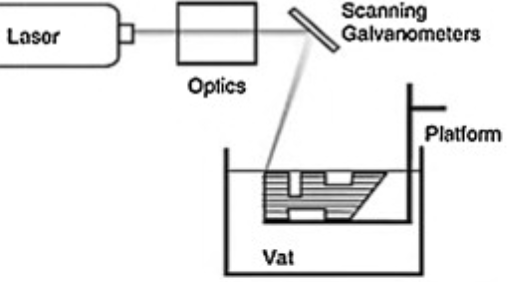
\includegraphics[scale=0.5]{Stereolitography-Scanner.png}
	\caption{Estereolitografia por Escaneamento}
\end{figure}

Entretanto, quando se trata de peças grandes, ao se utilizar um espelho galvanométrico, pode haver desfoque do feixe luminoso, dado que a distância entre o espelho e a superfície da resina não é constante (\cite{Huang2020}). 
Por isso, outra forma de realizar o escaneamento é manter o laser focado em um ponto fixo, e movimentar o recipiente de resina juntamente com a plataforma e o objeto impresso no plano XY, mantendo constante a distância entre a resina e o foco luminoso:

\begin{figure}[H]
	\centering
	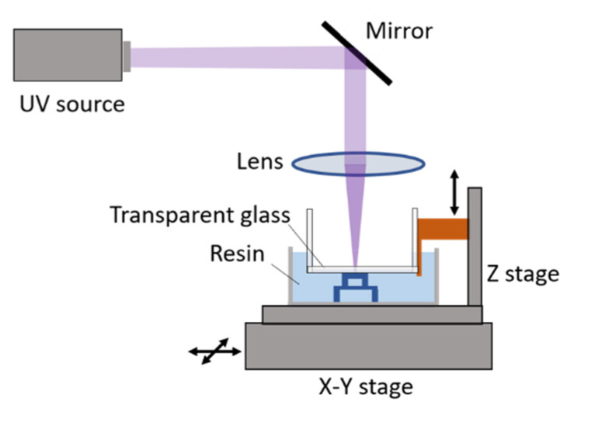
\includegraphics[scale=0.5]{Stereolitography-Scanner-XY.png}
	\caption{Estereolitografia por Escaneamento com plataforma móvel}
\end{figure}

Todavia este procedimento traz dificuldades quanto a resolução do movimento da plataforma que deve ser considerado. 

De forma geral, a estereolitografia por escaneamento produz peças com resolução impressionante (6 - 140 micrômetros) , sendo a opção comercial disponível com a maior capacidade de detalhamento do mercado. (\cite{Schmidleithner2016})
}

\item {Estereolitografia por Projeção:

O procedimento de Estereolitografia por Projeção se baseia na utilização de um modulador espacial de luz (Spatial Light Modulator, ou SLM), para curar uma camada de resina de forma integral. Na prática, dois modelos de SLM são utilizados:

\begin{enumerate}
	\item Emissivo: neste caso são utilizados painéis LCDs, entretanto a resolução da peça é dependente da resolução do dispositivo, além de que painéis LCD comerciais não emitem luz ultravioleta com alta intensidade atingindo apenas 12,5\% de eficiência (\cite{Sun2005}); 
	\item Reflexivo: onde são usados Cristal Líquido em Silício (liquid crystal on silicon, LCoS) ou Dispositivos Microespelhos Digitais (DMDs). Tais dispositivos, conseguem refletir luz ultravioleta com alta eficiência (88\% \cite{Sun2005}).
\end{enumerate}

Além dos dois métodos acima, existem ainda procedimentos emergentes mais complexos como a Estereolitografia Contínua (CLIP) e a Estereolitografia Volu-métrica que trazem algumas vantagens sobre os demais.
(\cite{Huang2020}) 
}
\end{enumerate}

\subsection{Selective Laser Sintering (SLS)}

\paragraph{}
A Sinterização Seletiva a Laser (SLS) utiliza um laser de alta potência direcionado com o auxílio de espelhos para um reservatório de pó de matéria prima. Tal laser une as partículas de material formando um objeto, uma camada por vez. Sempre que uma camada é concluída um dispositivo (roller ou sweeper) passa por sobre o reservatório principal, espalhando uma fina camada de pó para ser sinterizado na próxima iteração (\cite{Cheepu2021}).

\begin{figure}[H]
	\centering
	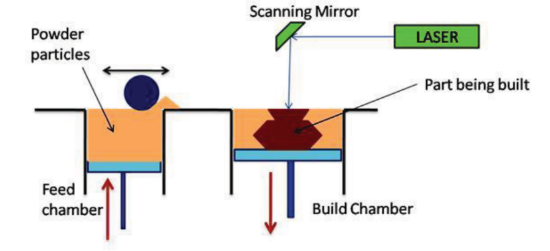
\includegraphics[scale=0.8]{SLS.png}
	\caption{Sinterização Seletiva a Laser}
\end{figure}

A SLS tem como objetivo principal garantir que o agrupamento entre as partículas formantes do objeto seja forte. Para tal, existem algumas formas de realizar este agrupamento:

\begin{enumerate}[leftmargin=*, listparindent=0.7cm]
	\item {
		Sinterização de estado sólido:

		É definido pela união que ocorre quando a temperatura atingida no material está entre metade da temperatura de fusão e a temperatura de fusão. Neste processo é formado um “pescoço” de matéria entre as partículas, não garantindo máxima densidade:

		\begin{figure}[H]
			\centering
			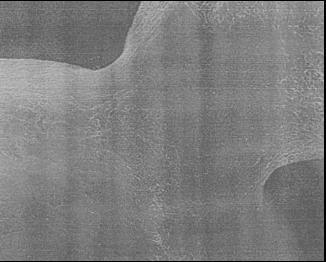
\includegraphics[scale=0.8]{SLS-neck.png}
			\caption{Sinterização Seletiva a Laser - "Pescoço"}
		\end{figure}

	}
	\item {
		Agrupamento quimicamente induzido:

		Ocorre quando o material submetido a sinterização, quando aquecido, reage quimicamente com o ambiente ou consigo mesmo criando um “agrupador”. Alguns exemplos:

		\begin{itemize}
		\item O material cerâmico SiC, quando aquecido na presença de O2, produz SiO2, que age como um aglomerante para moléculas SiC;
		\item O alumínio, quando aquecido na presença de N2, produz AlN, que age como um aglomerante para partículas de alumínio;
		\end{itemize}

	}

	\item{
		Sinterização de fase líquida ou derretimento parcial:

		A maioria dos processos que se enquadram nesta categoria envolvem liquefação completa de um aglomerante, através do aquecimento, misturado com partículas do material próximas do ponto de fusão. (cite)

	}
	\item{
	Derretimento total:

	Este processo consiste em utilizar alta potência no laser para derreter o material por completo, fazendo com que a densidade do objeto final seja a máxima possível para o material.
	}
\end{enumerate}

Os principais parâmetros a serem considerados para a SLS são a potência e a velocidade do laser, que fazem parte da equação da Densidade de Energia:

\[\textrm{Densidade de Energia (ED)} = \dfrac{\textrm{LP}}{\textrm{SS} \times \textrm{BS}} \;\; \mathbf{J}/\textrm{mm}^2 \]

Na equação acima LP (\emph{laser power}) é a potência do laser , SS (\emph{scan spacing}) é o espaçamento do escaneamento  e BS (\emph{beam speed}) é a velocidade do laser.

Estes parâmetros são importantes pois, para cada tipo de material, é necessário definir (geralmente de forma empírica) qual densidade de energia produz o melhor resultado (\cite{Goodridge2012}).

\subsection{Fused Deposition Modeling (FDM)}

\paragraph{}
O processo de Modelagem por Deposição de material Fundido (FDM) consiste em derreter material sólido (geralmente um termoplástico, polímero ou compósito) e o depositar, camada por camada, construindo um objeto.
De forma geral, as máquinas FDM são compostas por:

\par
Uma plataforma para impressão, geralmente com aquecimento controlado;
Um cabeçote aquecido para fusão e deposição do material;
Estruturas mecânicas para movimentação triaxial;

\par
Como este processo é o foco desta monografia, as seções abaixo discutem com mais detalhes cada parte da máquina.


\subsubsection{Mecânica: Movimentação do Efetuador}

\paragraph{}
A mecânica de uma impressora FDM deve implementar três eixos de liberdade, sendo eles independentes ou não. Algumas implementações para o dispositivo são:

\begin{enumerate}[leftmargin=*, listparindent=0.7cm]
	\item {
	Cabeçote móvel em XZ e mesa móvel em Y (XZ-Head):

	Esta mecânica realiza movimentos com a mesa no eixo Y e com o cabeçote de impressão em X e Z. É bastante comum nas impressoras 3D de entrada como as Ender 3, e também nas hobbystas como a RepRap Prusa i3


	\begin{figure}[H]
		\centering
		\begin{minipage}{.5\textwidth}
			\centering
			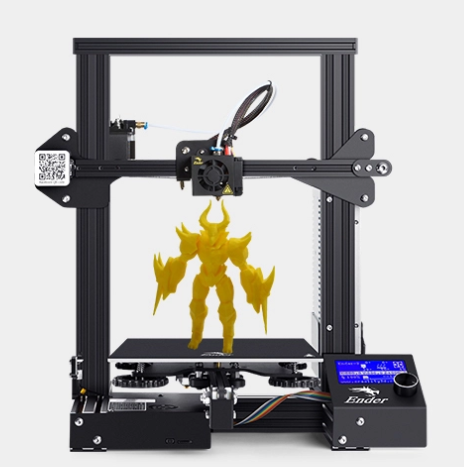
\includegraphics[height=.8\linewidth]{Ender3.png}
			\captionof{figure}{Ender 3 (\cite{ENDER3})}
			\label{fig:test1}
		\end{minipage}%
		\begin{minipage}{.5\textwidth}
			\centering
			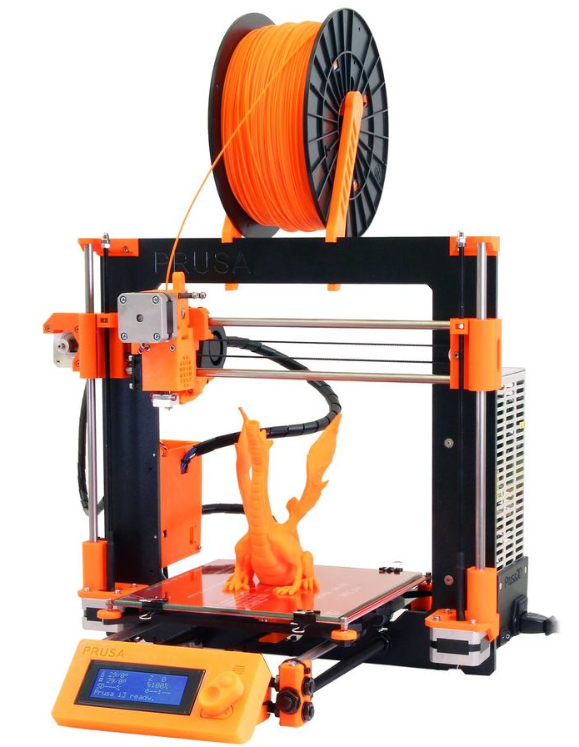
\includegraphics[height=.8\linewidth]{PrusaI3.png}
			\captionof{figure}{Prusa i3 (\cite{PRUSAI3})}
			\label{fig:test2}
		\end{minipage}
	\end{figure}

	Este tipo de dispositivo se destaca quanto a simplicidade de construção e funcionamento, mas traz consigo um problema de difícil solução: a massa movimentada em Y compreende a mesa e o objeto, o que aumenta o momento de inércia do eixo, intensificando as vibrações. (\cite{RINGING})

	O efeito causado pelas vibrações pode ser reduzido, diminuindo a velocidade de impressão, mas nunca eliminado. Em termos gerais, quanto menor a massa móvel de cada eixo, menos vibração e maior a qualidade e velocidade de impressão.

	}
	\item {
		Cabeçote móvel em XY e mesa móvel em Z
		
		Caracterizada por impressoras cujo cabeçote se move no plano XY e a mesa se move verticalmente, estas impressoras tendem a reduzir o problema da vibração, dado que a massa móvel do cabeçote é relativamente pequena, em comparação com a massa da mesa. 
		
		Existem algumas implementações para o movimento do cabeçote: 

		\begin{enumerate}[leftmargin=*, listparindent=0.7cm]
			\item {
				Cartesian XY-Head:
				
				São impressoras que usam os motores para mover eixos X e Y independentemente (\cite{Makksu2016}):
				
				\begin{figure}[H]
					\centering
					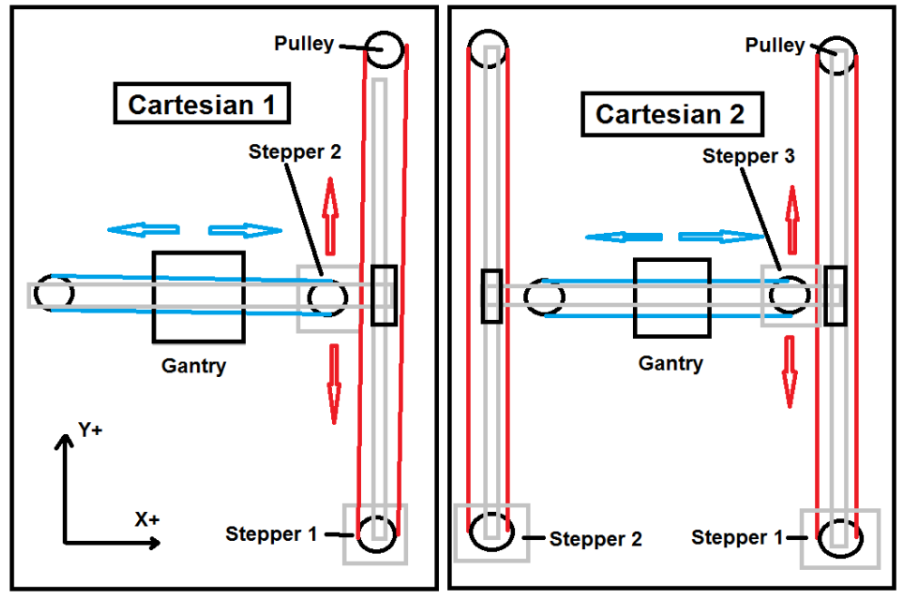
\includegraphics[height=.4\linewidth]{FDM-Cartesian.png}
					\caption{FDM do tipo Cartesian XY-Head}
				\end{figure}
		
				No exemplo acima vemos duas implementações possíveis: uma com um motor para cada eixo e outra com dois motores sincronizados para o eixo X e outro para o eixo Y.

				É importante salientar que nesta configuração, pelo menos um dos motores sempre vai estar em movimento junto ao seu eixo. Isso aumenta a massa móvel do conjunto e pode intensificar as vibrações.

				A Creality Ender 5 Pro é um exemplo de impressora 3d comercial que utiliza esta implementação:

				\begin{figure}[H]
					\centering
					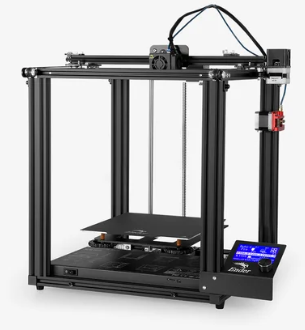
\includegraphics[height=.4\linewidth]{Ender5-pro.png}
					\caption{Ender 5 Pro (\cite{ENDER5PRO})}
				\end{figure}
					
			}
			\item {
				H-Bot:
				
				Nesta implementação os dois motores atuam em conjunto com um sistema de correia e polias para mover o cabeçote no plano XY. Este sistema utiliza uma longa correia, presa no cabeçote (\cite{Sollmann2010}).

				\begin{figure}[H]
					\centering
					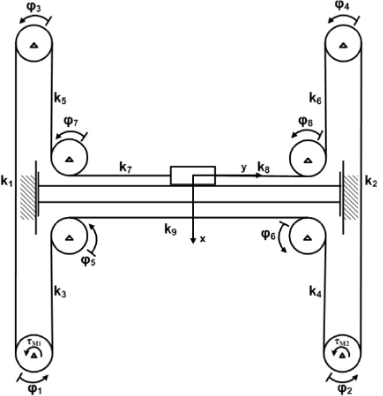
\includegraphics[height=.4\linewidth]{FDM-Hbot.png}
					\caption{FDM H-Bot}
				\end{figure}

				É importante notar que os motores são estacionários e que a rotação de apenas um motor provoca um movimento em 45º no cabeçote. O movimento do efetuador pode ser descrito com a seguinte expressão:

				\[ 
					\begin{bmatrix}
						\Delta x \\
						\Delta y
					\end{bmatrix} 
					=	
					\begin{bmatrix}
						-\dfrac{1}{2}r & \dfrac{1}{2}r \\[2ex]
						-\dfrac{1}{2}r & -\dfrac{1}{2}r
					\end{bmatrix} 
					\times
					\begin{bmatrix}
						\Delta \varphi_{1} \\
						\Delta \varphi_{2}
					\end{bmatrix} 
				\]
					
				Na qual $\Delta x$ e $\Delta y$ são variações de movimento do cabeçote, $\Delta \varphi_{1}$ e $\Delta \varphi_{2}$ são as rotações dos motores e $r$ é o raio das polias dos motores (assumindo iguais) (\cite{Sollmann2010})

				Esta implementação apresenta uma fraqueza: o movimento do efetuador é gerado por uma única correia, provocando torque indesejado na estrutura do cabeçote (\cite{Makksu2016}).
			}
			\item {
				Core-XY:
				
				Bastante semelhante com a H-Bot, a implementação Core-XY utiliza dois conjuntos de correia e polias para movimentar o efetuador no plano XY. A equação de movimento do cabeçote é idêntica à anterior. 

				\begin{figure}[H]
					\centering
					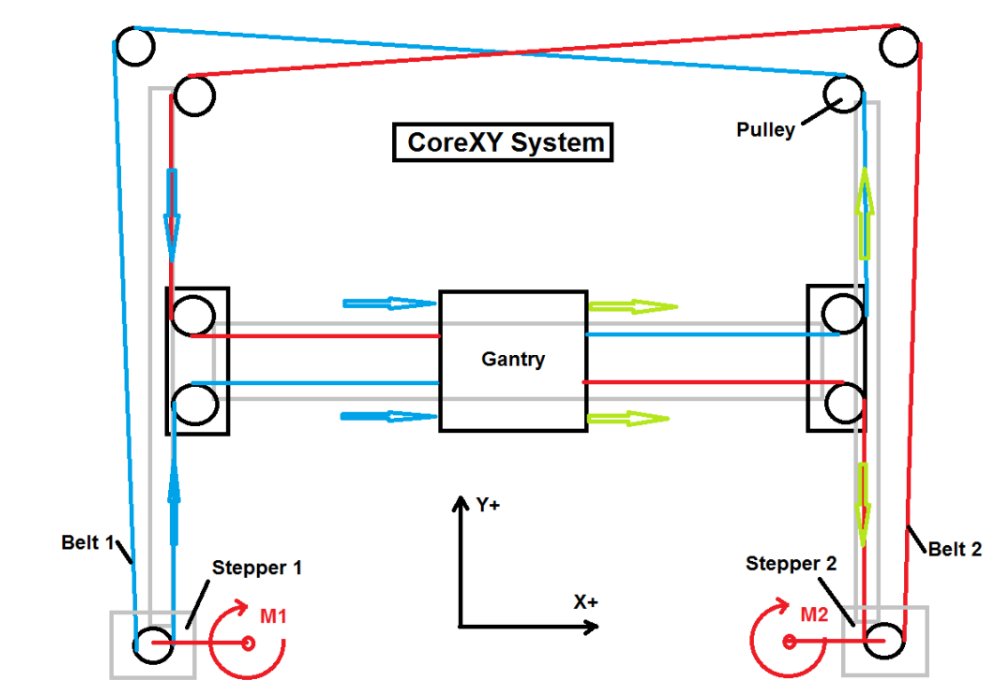
\includegraphics[height=.4\linewidth]{FDM-CoreXy.png}
					\caption{FDM Core-XY}
				\end{figure}
				
				A mudança mais importante que essa implementação proporciona é a eliminação do torque no efetuador, que agora é distribuído pelos dois conjuntos de correias (\cite{COREXY}).
				
			}
		\end{enumerate}
	}

	Além da movimentação no plano XY, estas impressoras necessitam de permitir movimento no eixo Z, da plataforma de impressão. Algumas implementações sugeridas para esta movimentação são:

	\begin{enumerate}[leftmargin=*, listparindent=0.7cm]
		\item {
			
			Cantilever: 
				
			A mesa de impressão é apoiada e movida somente por um de seus lados. Essa implementação, apesar de usada em alguns modelos comerciais como a nacional GTmax3d Core A3 e a Cubex Duo (\cite{CUBEXDUO}), requer uma estrutura mecânica robusta para sustentar a plataforma e evitar folgas e inclinações indesejadas.

			\begin{figure}[H]
				\centering
				\begin{minipage}{.5\textwidth}
					\centering
					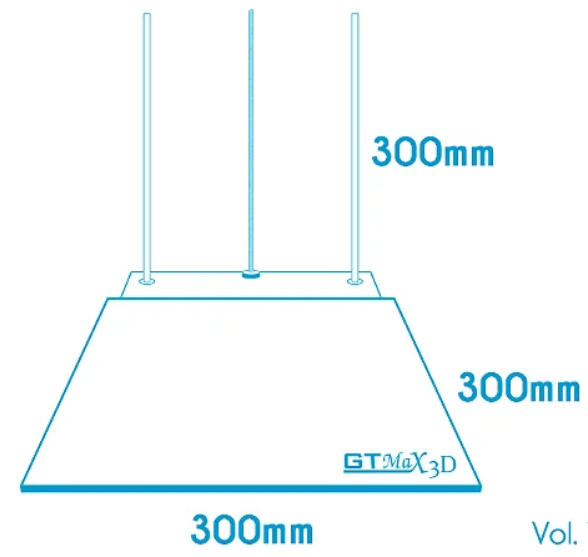
\includegraphics[height=.8\linewidth]{GTMAX3d.png}
					\captionof{figure}{GTmax3d Core A3 }
					\label{fig:gtmax3d}
				\end{minipage}%
				\begin{minipage}{.5\textwidth}
					\centering
					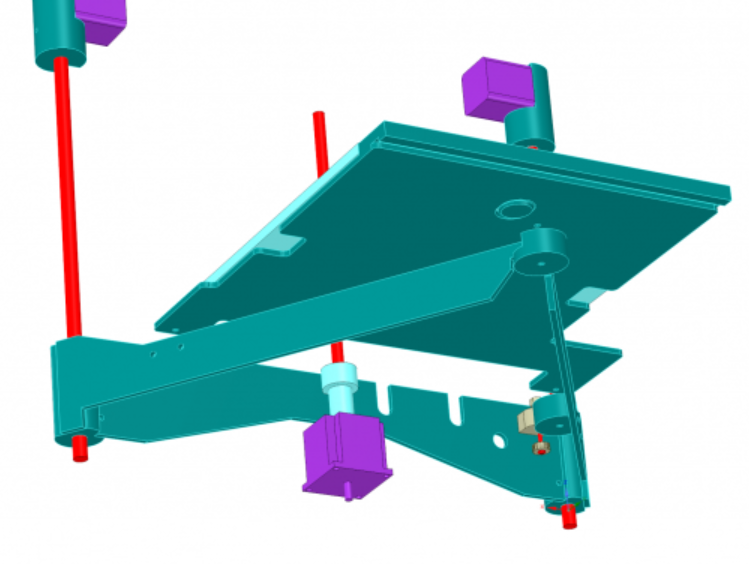
\includegraphics[height=.8\linewidth]{CubeX.png}
					\captionof{figure}{Cubex Duo 1}
					\label{fig:cubexduo}
				\end{minipage}
			\end{figure}

			}
			\item {
			Bi-apoiada:
			
			Nesta implementação a mesa de impressão é apoiada em dois lados, trazendo mais estabilidade em pelo menos um dos eixos de inclinação. A Creality Ender 5 Plus é um exemplo desta implementação:
			
			 
			\begin{figure}[H]
				\centering
				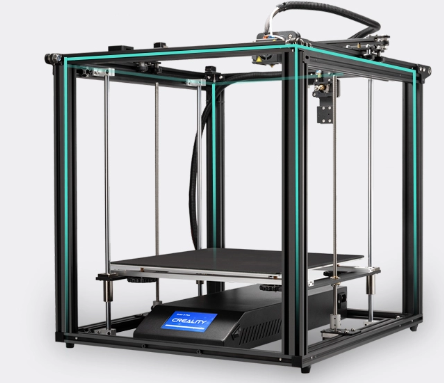
\includegraphics[height=.4\linewidth]{Ender5-Plus.png}
				\caption{Ender 5 Plus {\cite{ENDER5PLUS}}}
			\end{figure}

			}
			\item {
			Triapoiada:
			
			Nestes dispositivos a plataforma de impressão é apoiada em 3 pontos distintos, aumentando a estabilidade em dois eixos de inclinação. Comercialmente, apenas impressoras de topo de linha como a Bambu Lab X1 implementam este modelo.
				
			\begin{figure}[H]
				\centering
				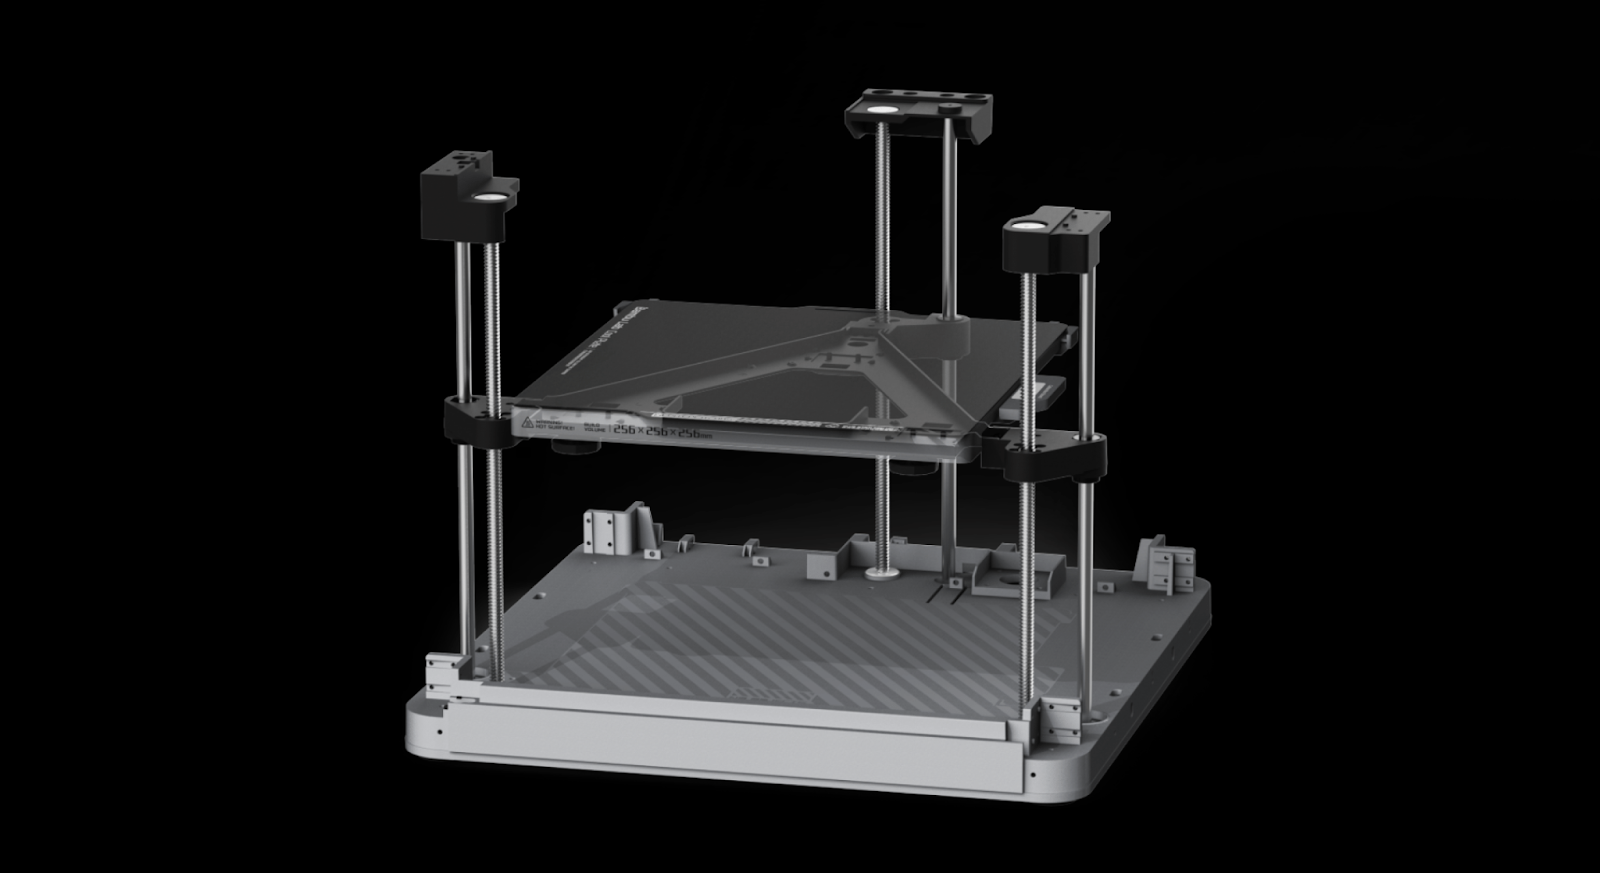
\includegraphics[height=.4\linewidth]{BambuLab-X1.png}
				\caption{BambuLab X1 {\cite{BAMBULAB}}}
			\end{figure} 

		}
	\end{enumerate}

	\item {
		Impressora de Esteira
		
		A impressora de esteira é uma implementação especial que substitui a mesa fixa do equipamento padrão por uma esteira rolante. Essa modificação possibilita impressão “infinita” no eixo longitudinal, por apresentar os seus eixos de maneira não ortogonal. (\cite{Whelan2018}) 

		
		Neste modelo o eixo “infinito” é posicionado a 45º do que seria equivalente ao plano XY de uma impressora convencional. Como exemplo comercial temos a Creality CR-30 e a Blackbelt:
		
		\begin{figure}[H]
			\centering
			\begin{minipage}{.5\textwidth}
				\centering
				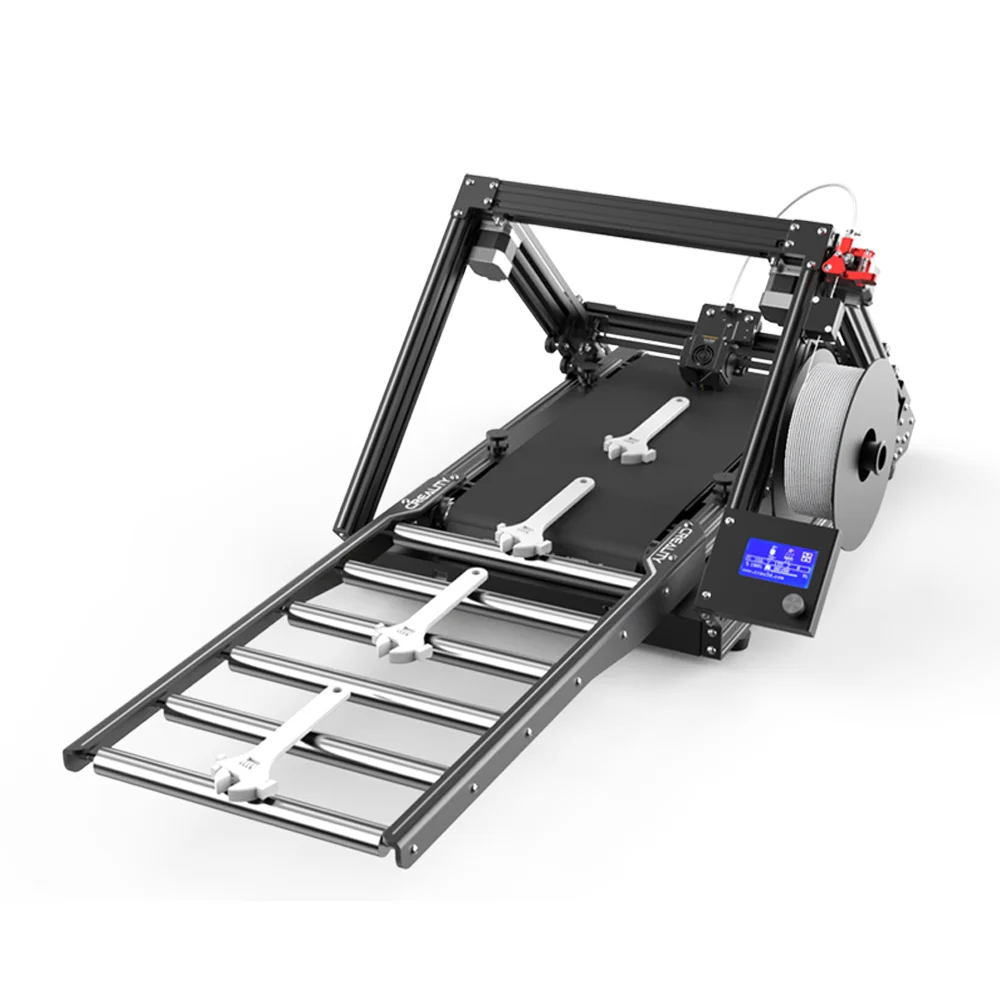
\includegraphics[height=.8\linewidth]{CR30.png}
				\captionof{figure}{CR-30 (\cite{CR30})}
				\label{fig:cr30}
			\end{minipage}%
			\begin{minipage}{.5\textwidth}
				\centering
				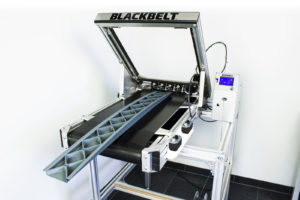
\includegraphics[height=.8\linewidth]{Blackbelt.png}
				\captionof{figure}{Blackbelt (\cite{BLACKBELT})}
				\label{fig:blackbelt}
			\end{minipage}
		\end{figure}

		Este modelo apresenta alguns desafios quanto à sua construção, em particular a dificuldade de manter e garantir o aquecimento da esteira de impressão. Tal desafio pode ser resolvido com esteiras especiais que suportam e melhor distribuem o calor por toda a superfície (\cite{ALL3DP:Belt3DPrinter}).  

	}
	\item {
		
		Impressora Delta
			
		Os modelos de impressora Delta se baseiam no funcionamento de um robô Delta (\cite{Florin2016}) tais como o IRB 360 FlexPicker da ABB:

		\begin{figure}[H]
			\centering
			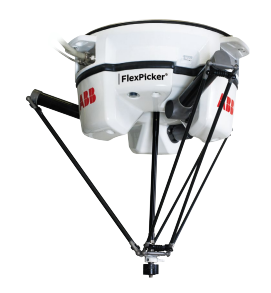
\includegraphics[height=.4\linewidth]{ABB-IRB360.png}
			\caption{ABB IRB 360 (\cite{ABB:IRB360})}
		\end{figure} 
		
		A mecânica consiste em suportar o efetuador por três hastes móveis, que por sua vez se acoplam em três barras fixas que possibilitam o seu movimento através de motores e correias ou fusos (\cite{Aasvik2017}).

		\begin{figure}[H]
			\centering
			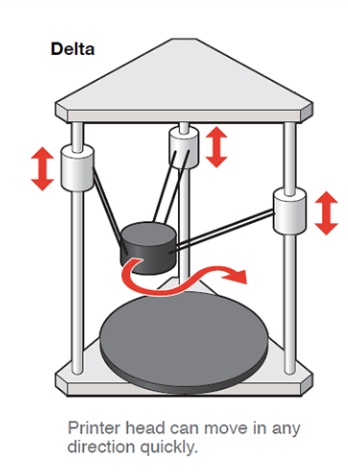
\includegraphics[height=.4\linewidth]{FDM-Delta.png}
			\caption{FDM Delta}
		\end{figure} 

		Apesar de interessante, a implementação apresenta desafios quanto à qualidade de impressão e ao tamanho do volume útil dos equipamentos (\cite{3DPRINTERLY}). 
	}
	\item {
		Polar
	
		A impressora Polar utiliza uma base rotativa e implementa geometria cilíndrica com três eixos: $\theta$ de rotação da base, R de raio do efetuador e Z de altura do efetuador. 

		A vantagem deste método, ainda pouco utilizado, é o bom espaço útil para impressão em relação ao tamanho da máquina, entretanto, existem alguns desafios quanto a resolução da impressão em plataformas com grande raio. Tal dificuldade advém do fato de que, para um passo angular constante de um motor, quanto maior o raio do disco, maior a distância linear deslocada (\cite{Deshpande2019}). 
	}
	\item {
		Manipulador Robótico

		Esta categoria de implementações busca utilizar modelos de manipuladores robóticos da indústria, como por exemplo os Selective Compliance Assembly Robot Arm (SCARA), para realizar a tarefa de manufatura aditiva. 

		Os robôs SCARA, mais comumente utilizados para a impressão 3d, são manipuladores compostos por duas juntas rotativas e uma prismática (\cite{Koo2019}). 

		\begin{figure}[H]
			\centering
			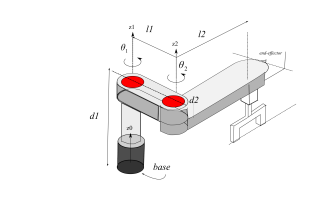
\includegraphics[height=.4\linewidth]{SCARA.png}
			\caption{Robô SCARA}
		\end{figure} 
		
		Abaixo estão alguns exemplos de implementação (\cite{ALL3DP:SCARA3DPrinter} e \cite{POTTERSCARA}):

		\begin{figure}[H]
			\centering
			\begin{minipage}{.5\textwidth}
				\centering
				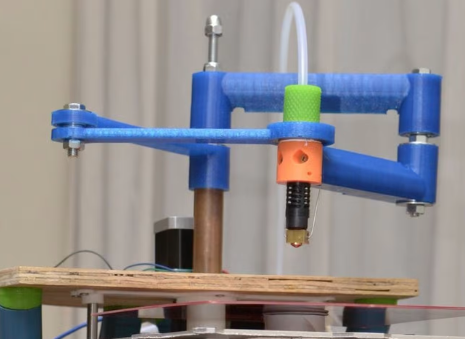
\includegraphics[height=.8\linewidth]{FDM-Scara.png}
				\captionof{figure}{FDM SCARA}
				\label{fig:fdmscara}
			\end{minipage}%
			\begin{minipage}{.5\textwidth}
				\centering
				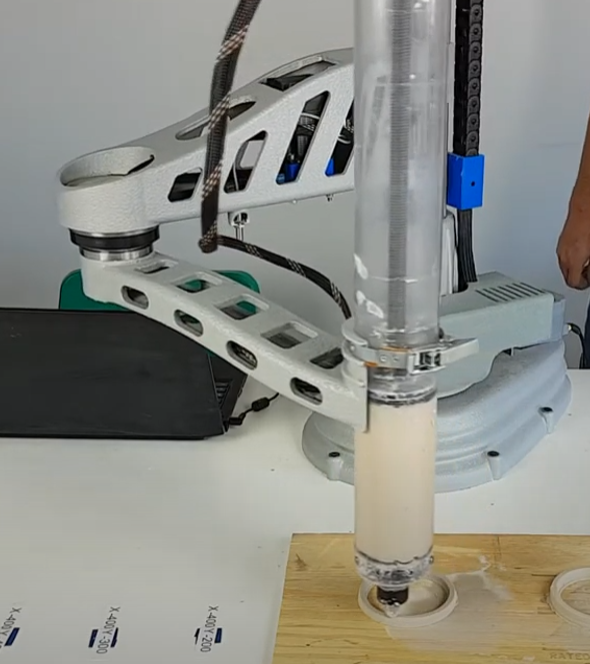
\includegraphics[height=.8\linewidth]{FDM-Scara-Potter.png}
				\captionof{figure}{FDM SCARA Cerâmica}
				\label{fig:potter}
			\end{minipage}
		\end{figure}

		A implementação com o SCARA bot trás complicações nas operações de controle para a tarefa e requer alta precisão de juntas e baixa massa de efetuador para garantir um nível de qualidade satisfatório. Apesar disso, traz flexibilidade quanto a área de impressão e mobilidade, sendo consideradas inclusive implementações com base móvel: 

		\begin{figure}[H]
			\centering
			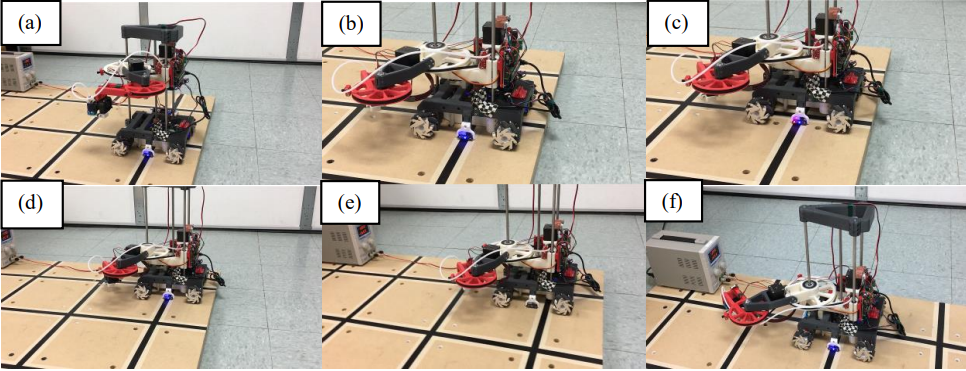
\includegraphics[height=.4\linewidth]{FDM-Scara-Mobile.png}
			\caption{FDM SCARA com base móvel}
		\end{figure} 

	}
\end{enumerate}

\subsubsection{Mecânica: Extrusor de Filamento}

\paragraph{}
Além do desafio de mover a cabeça de impressão, implementações de impressoras 3D FDM tem que alimentar um filamento de material polímero através do bico, para formar o objeto. O dispositivo que realiza esta tarefa é chamado extrusor. Algumas metodologias sugeridas para o desenvolvimento de extrusores serão discutidas a seguir.

\begin{enumerate}
	\item {
		Direct Extruder:
		
		O termo Direct Extruder (ou extrusor direto) caracteriza implementações que posicionam o mecanismo extrusor diretamente sobre a cabeça de impressão (\cite{FILAMENT2PRINT} e \cite{RECREUS}). 


		
		Essa categoria de extrusores traz grande versatilidade quanto a quantidade de materiais possíveis de serem impressos, facilitando a impressão de materiais maleáveis e flexíveis. Entretanto, agrega ao efetuador a massa de um motor e mecanismos, intensificando vibrações se for movimentado rapidamente (\cite{ALL3DP:3DPrinterExtruder}).
		
	}
	\item {
		Bowden Tube Extruder

		Os extrusores do tipo Bowden Tube ganham este nome devido ao aparato Bowden Cable (ou cabo de Bowden) no qual um fio de material é passado por dentro de um tubo flexível com o objetivo de transmitir potência mecânica (\cite{Letier2006}). Tal mecanismo tem ampla adoção na indústria, desde a atuação de freios de bicicleta até robôs para operações cirúrgicas (\cite{Jeong2015}). 

		No caso dos extrusores Bowden Tube, o filamento de polímero é empurrado por um tubo (geralmente de PTFE \cite{PTFE}) até chegar ao bico da impressora 3D. 
		
		\begin{figure}[H]
			\centering
			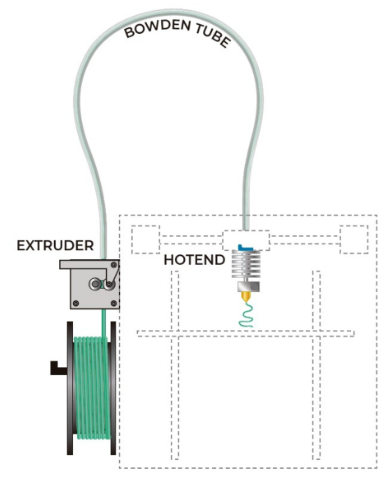
\includegraphics[height=.4\linewidth]{Bowden-extruder.png}
			\caption{Extrusora Bowden}
		\end{figure} 
		
		Este modelo permite maiores velocidades de impressão, devido a redução de massa no efetuador, porém alguns materiais podem apresentar dificuldade para serem impressos, por causa do atrito gerado pelo tubo de Bowden, como é o caso dos materiais flexíveis. Uma outra dificuldade causada pelo atrito é a sobrecarga do motor de extrusão, que pode necessitar de um mecanismo adicional para atingir o torque necessário para mover o filamento (\cite{ALL3DP:3DPrinterExtruder}).

	}	
\end{enumerate}	

Quanto ao mecanismo que realiza o movimento do filamento, existem duas implementações mais usadas: movimentação direta e engrenada. Na primeira o motor é acoplado a uma engrenagem dentada que arrasta o filamento diretamente. Na segunda, o acoplamento é feito a uma caixa de engrenagens, que amplifica o torque gerado pelo motor.

Ambas as implementações podem contar com  duas engrenagens dentadas, em lados opostos do filamento, rotacionando em sentidos opostos, objetivando aumentar a área de contato entre o filamento e as engrenagens.

\begin{figure}[H]
	\centering
	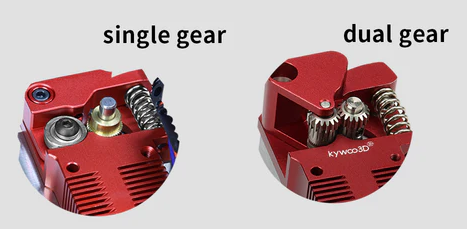
\includegraphics[height=.4\linewidth]{extruder-gear.png}
	\caption{Comparação dos mecanismos extrusores}
\end{figure}

\subsubsection{Termodinâmica: Bico Aquecido (Hot End)}

Considerada a parte mais desafiadora da construção de uma impressora 3D FDM, o bico aquecido tem a função de derreter o filamento de matéria prima de forma controlada (\cite{REPRAP:HotEndDesignTheory}, imagem \cite{FILAMENT2PRINT}).

\begin{figure}[H]
	\centering
	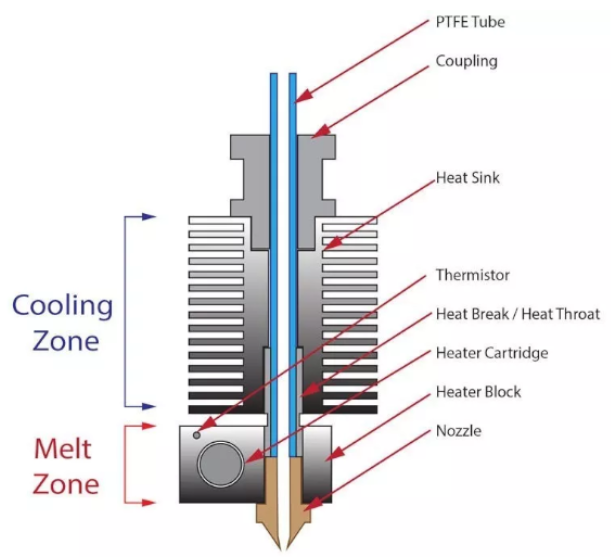
\includegraphics[height=.4\linewidth]{hot-end.png}
	\caption{Partes do bico aquecido (Hot End)}
\end{figure}

A estrutura básica de um bico aquecido tem os seguintes elementos: bloco aquecido, separador térmico, dissipador, elemento aquecedor, sensor de temperatura e bocal.
	
\begin{enumerate}
	\item {
		Bloco térmico: 
		
		E fabricado de material bom condutor de calor e objetiva conduzir o calor gerado pelo elemento aquecedor o bocal e derreter o filamento;
	}
	\item {
		Separador Térmico: 
		
		Tem como função desacelerar a condução de calor para o restante do filamento, já que este, denominado “heat creep” pode fazer o filamento se liquefazer antes de chegar ao bocal, podendo causar entupimento do bico aquecido e prejudicar a qualidade de impressão (\cite{ALL3DP:HowtoFixHeatCreep}). 
	}
	\item {
		Dissipador: 
		
		Objetiva acelerar a dissipação do calor que é conduzido pelo separador térmico. Tal efeito pode ser acelerado com a aplicação de ventilação ativa sobre o dissipador (\cite{ALL3DP:HowtoPreventHeatCreep}) 
	}
	\item {
		Elemento aquecedor: 
		
		De forma geral, se trata uma resistência pela qual, por Efeito Joule, é convertida potência elétrica em térmica (\cite{Passos2009}).
		
	}
	\item {
		Sensor de Temperatura: 
		
		Se trata de um aparelho capaz de aferir a temperatura do bloco aquecido, podendo ser um termopar, termistor ou outro instrumento que realiza tal função. É de grande importância que este elemento esteja presente no bico aquecido, para que a malha de controle de sua temperatura possa ser fechada.
	}
	\item {
		Bocal:  
		
		É o elemento final da cadeia de aquecimento da matéria prima, responsável por contrair o material derretido até o diâmetro final esperado. A escolha do diâmetro do bocal altera o fluxo de material, assim como a largura mínima das paredes do objeto impresso.
	}
\end{enumerate}

Algumas versões comerciais de bico aquecido são a E3D V6 e a E3D Hemera, a última inclusive incorpora um sistema Direct Drive (\cite{V6} e \cite{HEMERA}).

\begin{figure}[H]
	\centering
	\begin{minipage}{.5\textwidth}
		\centering
		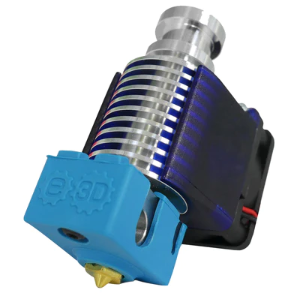
\includegraphics[height=.8\linewidth]{V6.png}
		\captionof{figure}{Hot-end V6}
		\label{fig:v6}
	\end{minipage}%
	\begin{minipage}{.5\textwidth}
		\centering
		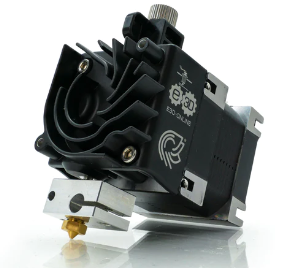
\includegraphics[height=.8\linewidth]{Hemera.png}
		\captionof{figure}{Hot-end Hemera}
		\label{fig:hemera}
	\end{minipage}
\end{figure}

\subsubsection{Termodinâmica: Mesa Aquecida (Heated Bed)}

\paragraph{}
A plataforma que suporta o objeto impresso deve ser aquecida objetivando desacelerar o seu resfriamento. O resfriamento rápido e mal distribuído do material pode causar defeitos de fabricação como empenamento e rachaduras (\cite{Douglas2021}).

\begin{figure}[H]
	\centering
	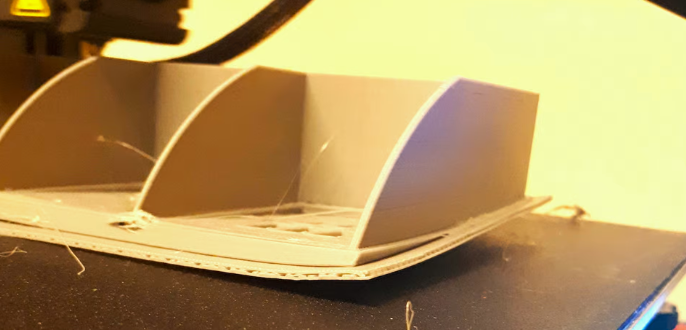
\includegraphics[height=.4\linewidth]{warping.png}
	\caption{Defeitos causados por não aquecer a mesa de impressão}
\end{figure}

O dispositivo é construído através de uma placa de material condutor de calor, acoplado a uma resistência elétrica para prover o calor necessário. É importante a utilização de um sensor de temperatura para realizar o controle da temperatura da mesa em malha fechada.

% 2.3.5 Elétrica e Eletrônica

% A parte elétrica/eletrônica da impressora 3D FDM compreende os seguintes componentes:

% Motores:
% Drivers para motores
% Sensores de temperatura
% Drivers para aquecedores (Resistências)
% Sensores de fim de curso
% Fonte
% Microcontrolador
% Outros


% 2.3.6 Firmware e Software

% O firmware de uma impressora 3D FDM deve ter como funcionalidades o controle e sensoriamento de todo o aparato da máquina além da leitura e interpretação de código de fabricação (GCode). Funcionalidades extras como interatividade com o usuário, acesso e visualização remota, detecção de falhas, compensação de vibrações são opcionais, no entanto podem aumentar a experiência de usuário e a qualidade final dos objetos.

% Funcionalidades Primárias
	
% As tarefas principais do firmware de uma impressora 3D FDM podem ser divididas em quatro categorias principais:

% Leitura e interpretação de código de fabricação (GCode)
% Sensoriamento
% Controle dos motores
% Controle dos elementos aquecidos

% Funcionalidades Extras

% 	A categoria de funcionalidades extras compreende funções opcionais que podem agregar de alguma forma na experiência de impressão. Não são obrigatórias para o funcionamento do equipamento, mas podem adicionar usabilidade e qualidade de impressão. Alguns exemplos são:

% Interatividade
% Detecção de falhas
% Compensação de vibrações






\printbibliography[title=Referências]

\end{document}